\chapter{État de l'art}

En effectuant nos recherches sur le sujet nous avons trouvé beaucoup d'informations sur les abeilles et le travail des apiculteurs en général, ainsi que des systèmes "maison" développés par des particuliers pour surveiller un peu mieux leurs ruches. Cependant nous avons également découvert l'existence de quatre projets similaires au notre: trois projets en cours ayant une approche OpenSource et un projet commercial déjà développé. Ce dernier appartient à la société anglaise Arnia. Ce système est décrit \cite{arnia} comme permettant à l'utilisateur d'avoir des informations sur une ou plusieurs ruches telles que la température, l'humidité et l'intensité acoustique dans la ruche ainsi que la température du couvain. Les apiculteurs peuvent ensuite visualiser ces informations sur une partie sécurisée du site internet d'arnia. Ils peuvent également comparer les informations et évolution d'une ou plusieurs ruches, comme on peut le voir sur la figure \ref{fig:arnia1}.

\begin{figure}[h]
\centering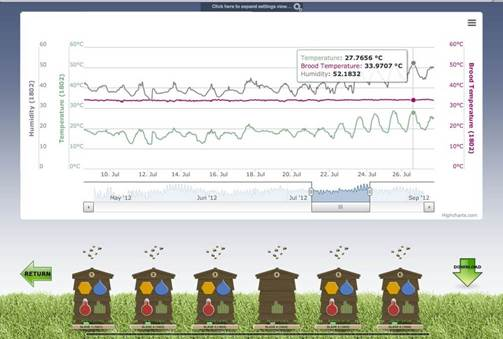
\includegraphics{arnia1.jpg}
\caption{\label{fig:arnia1} Interface du système d'arnia: comparaison des données d'une ruche}
\end{figure}

L'un des projets OpenSource est développé par Ken Meyer sur le site hackaday \cite{hackaday} et consiste à mesurer la température, l'humidité et le poids d'une ruche. Ce projet est encore en développement et plusieurs prototypes ont déjà été testés.

Il existe également un autre projet OpenSource sur le sujet. Il s'agit de Bzzz \cite{projetBzzz}, développé par le Fablab de Lannion. Ce système propose une supervision de la température intérieure, de la luminosité extérieure et la masse d'une seule ruche via un envoi de données périodique par SMS et par visualisation des données sur un portail en ligne. L'utilisateur pourra également configurer des alertes via le portail.

Enfin le dernier système existant que nous avons trouvé a été développé conjointement par le Fablab de Barcelone et Open Tech Collaborative, Denver, USA \cite{OpenBeehives}. Ce projet OpenSource, appelé Open Source BeeHive, ne s'adapte pas aux ruches classiques mais propose une architecture simple qui permet de construire sa propre ruche entièrement, comme on peut le voir sur les figures \ref{fig:OSBH2} et \ref{fig:OSBH}.

\begin{figure}[h]
\centering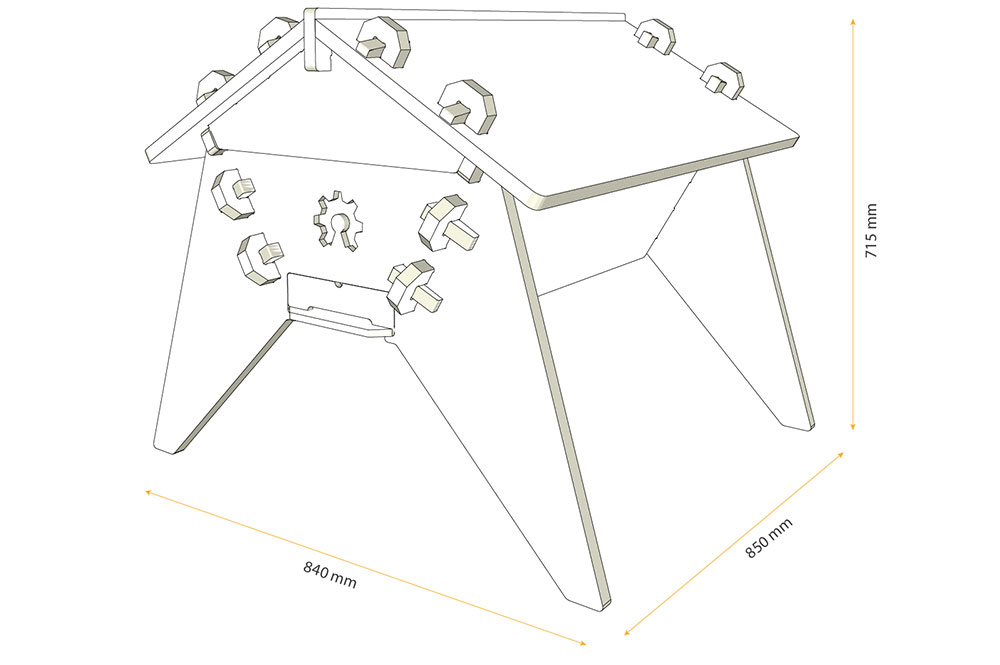
\includegraphics[scale=0.3]{OSBH.jpg}
\caption{\label{fig:OSBH} Modèle de ruche Open Source Beehive}
\end{figure}

\begin{figure}[h]
\centering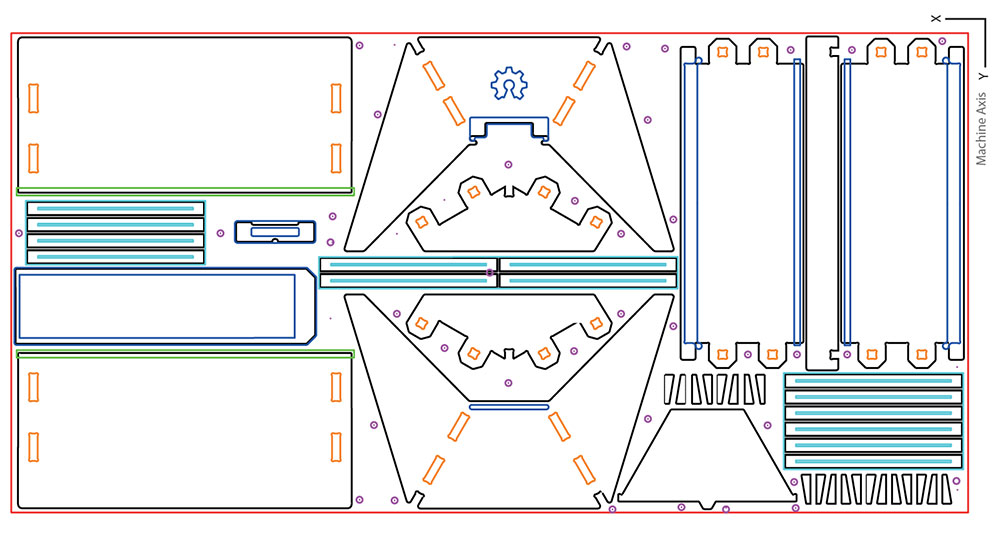
\includegraphics[scale=0.3]{OSBH2.jpg}
\caption{\label{fig:OSBH2} Plan de la ruche Open Source Beehive}
\end{figure}

Ensuite un kit de capteurs à installer permet de mesurer la température, l'humidité, l'intensité acoustique et le nombre d'abeilles via un capteur infrarouge. Les données seront ensuite visibles de tous sur la plateforme Smart Citizen.

Nous n'avons pas détaillé ici tous les projets que nous avons trouvés du fait de leur grand nombre. Cependant nous nous sommes intéressés à ceux qui présentaient un intérêt pour le système que nous voulons développer. 

Concernant le traitement sonore, le site internet Beesource comporte une description complète du système Apidictor \cite{apidictor}. Ce système permet de filtrer le son émit par une ruche pour prévoir un essaimage. Un schéma du montage électrique ainsi qu'un texte expliquant quelles fréquences sont surveillées et quelles méthodes ont été utilisées pour vérifier le bon fonctionnement de ce système sont également présents. Nous ne réutiliserons pas le montage proposé, car le traitement du signal sonore se fera de manière informatisée, en revanche le travail effectué pour savoir quelles fréquences sont à surveiller nous sera utile.

A propos de la transmission de l'information à l'apiculteur, deux moyens sont très souvent utilisés: un site internet sécurisé et une application pour smart-phone. Concernant le site internet, celui de la société Arnia nous a semblé complet et clair. Pour l'application smart-phone, l'entreprise américaine B-Ware en a mis une au point mettant bien en avant le tableau de bord, l'affichage de l'historique des paramètres de la ruche et la personnalisation des alertes en laissant même l'apiculteur définir lui même les seuils de déclenchement des avertissements comme nous pouvons le voir sur la figure \ref{fig:app}.   

\begin{figure}[h]
\centering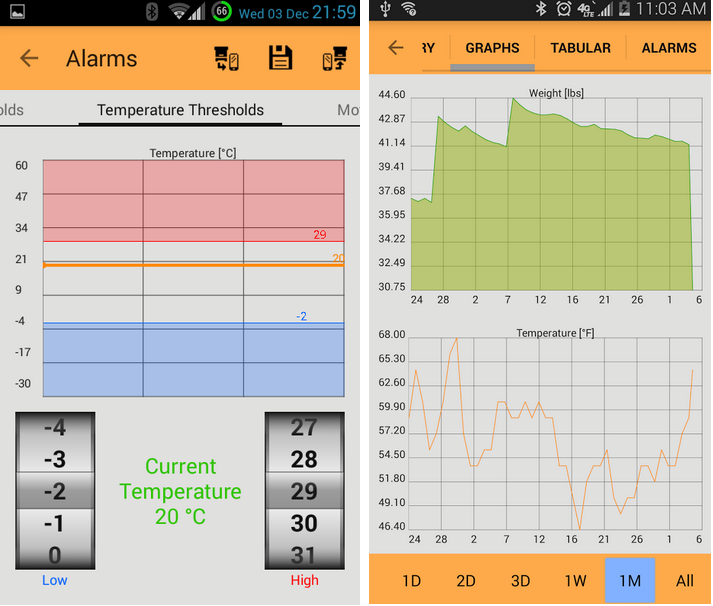
\includegraphics[scale=0.3]{Bee_app.png}
\caption{\label{fig:app} Capture d'écran de l'application B-Ware}
\end{figure} 

La société BeeWise d'origine française a développé un système d'alimentation écologique à l'aide de panneaux solaires connectés au Bee_monitor regroupant les cartes électroniques pour le traitement des données et de transmission. Il suffirai juste de la fixer sur le couvercle de la ruche en prenant soit d'étudier l'orientation adéquate au préalable comme sur la figure \ref{fig:solar}. Cette solution semble être la plus répandue car elle est également utilisée par les développeurs de l'ApiScan, un système de comptage de d'abeilles installé sur la planche d'envol pour minimiser la gène occasionnée.    

\begin{figure}[h]
\centering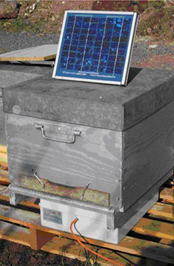
\includegraphics[scale=0.3]{solar.png}
\caption{\label{fig:app} Système de panneau solaire installé sur une ruche}
\end{figure} 

   